The software design was mainly guided by the provided format of the raw data. Which was from a few different sources, as different people were working with different data at the Hospital, and they did not have a unified collection. Thus the following documentation of the software design will be structured going from the raw data, to the preprocessed data, and then the model itself.

\section{Raw Data}

The raw data is scattered amongst many files, are registered in different spaces, does not have masks applied, along with other challenges detailed in \reflink{sec:preproc}{Section}.

\begin{figure}[H]
\centering
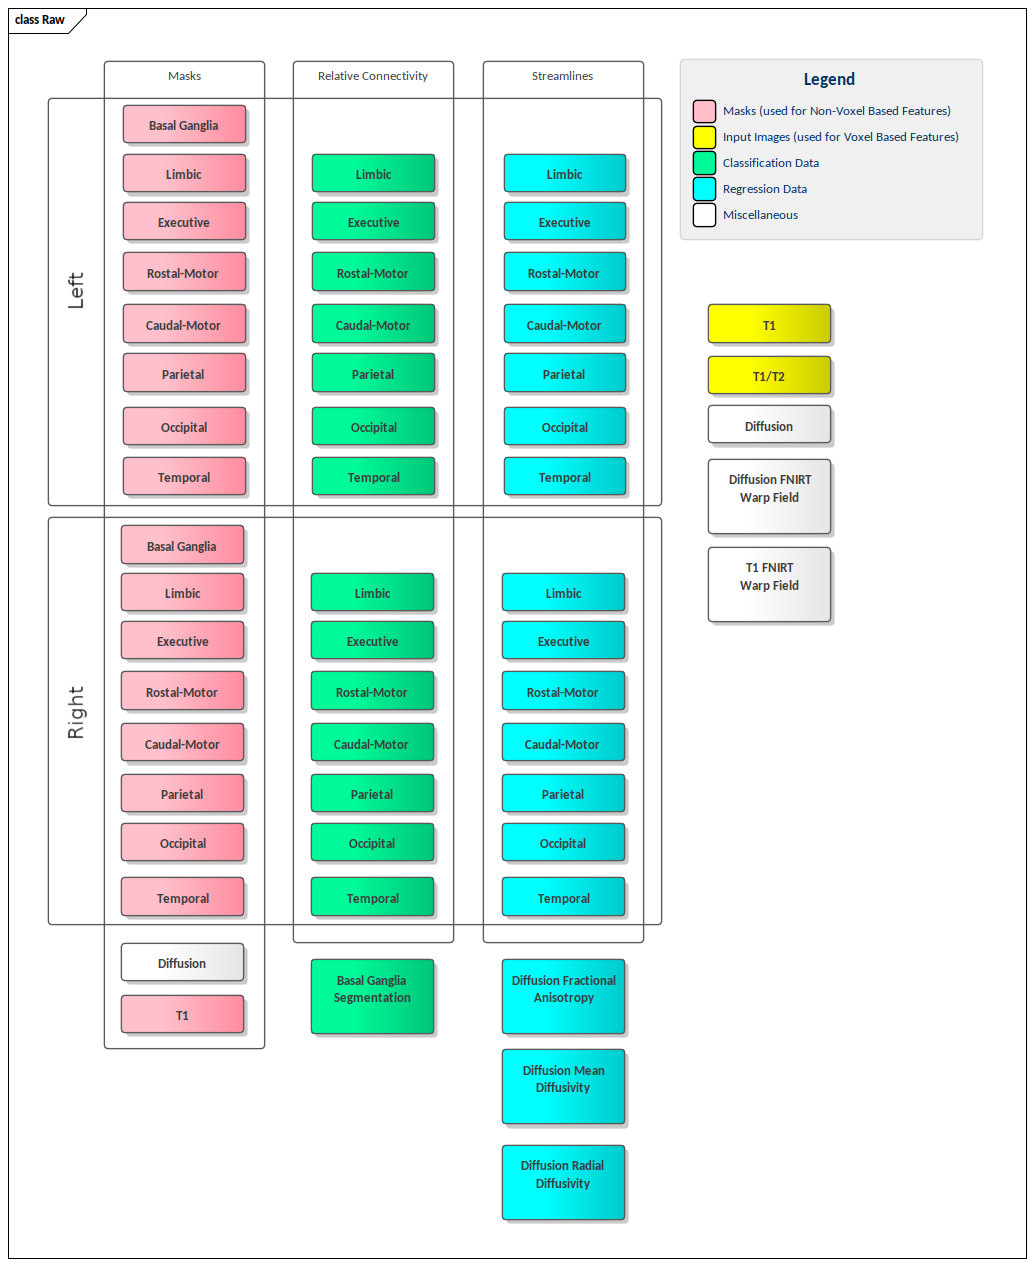
\includegraphics[width=0.7\textwidth]{DataRaw}
\caption{Files: Raw}
\end{figure}

The following class diagram documentations are detailed abstractions of the actual source code, as \ac{UML} is not completely Python compliant. Before moving on, the following simple data types are used in the \ac{UML} diagrams:

\begin{figure}[H]
\centering
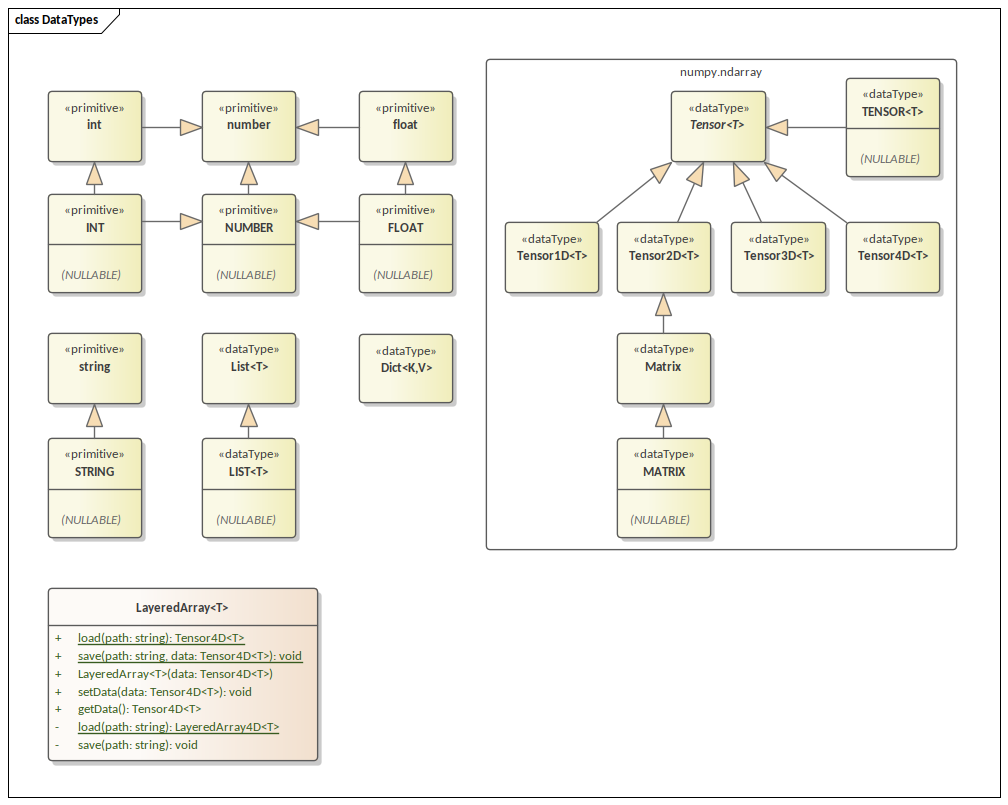
\includegraphics[width=0.7\textwidth]{ClassDataTypes}
\caption{Class Diagram: Data Types}
\end{figure}

There is one odd one out in this diagram, that being the LayeredArray, which is more than a simple data type or primitive. This class is a simple space efficient data structure of a 4D tensor.\par
Storing some of the data provided can be highly inefficient by storing the raw tensor. Ultimately the design aims to collect the scattered data from multiple files, into clean logical groups, for example all the cortical target masks into a single 4D tensor where the 4th dimension is reserved for the multiple targets. But this poses a greatly inefficient way of storing the data, as each target region only takes up a small portion of the entire space. The idea behind the LayeredArray class, it stores the 4D tensor as a list of 3D tensors, each cropped down to their effective space where there are non-zero voxels. This also requires an additional list of 3D vectors to store each layer's origin, and where to paste it in the original space.\par
This solution offers a very efficient way of storing data for this use case, as the raw storage solution for the cortical target masks were around 50MBs, and this cuts it down to 3MBs. This is even more drastic for the relative connectivity, which is more than a simple boolean mask and proportionally takes up even less space of the entire brain; in which's case it was cut down from 110MBs to 0.5MBs, reducing the disk requirement by several magnitudes.\par
The original \ac{NIfTI} format also does a very good job at storing data efficiently, but this solution provides control over the way of storing the data on a much lower level. This is beneficial as the data are stored in numpy format, making it easier to ignore certain data type safety checks, data type conversions, and leaving behind the \ac{NIfTI} format's additional complexity of the orientation, transformation, and many more nuances that are part of the \ac{NIfTI} header.\par
This has the undoubted drawback of not being able to use \ac{FSL} tools natively on our datatypes, such as fsleyes for simply viewing a record. But thanks to the opensource nature of the \ac{FSL} suite, with a few additional lines of code, support can be added for our datatypes (included in \reflink{apx:source}{Appendix}).

\begin{figure}[H]
\centering
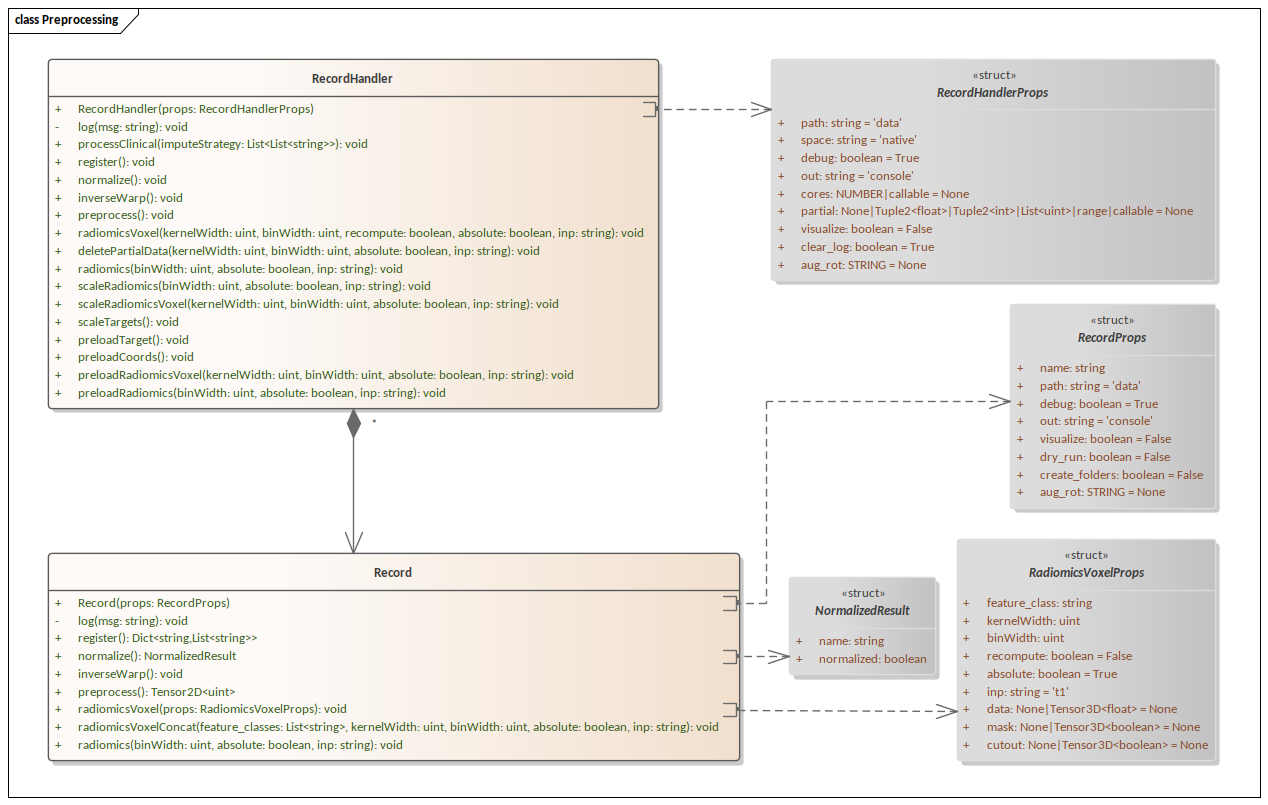
\includegraphics[width=0.7\textwidth]{ClassPreprocessing}
\caption{Class Diagram: Preprocessing}
\end{figure}

The class diagram above contains the two classes responsible for the preprocessing of the data. The RecordHandler being the controller itself that handles the high level operations on a collection of records. And the records handling the low level computations on the data itself.

\section{Common Functions}

There are set of static common functions, which give the low level backbone of the entire project. They are grouped into two categories, util and visual. Where the prior one contains everything from simple data type castings, external \ac{FSL} library system calls, to computing radiomics, and more. And the latter one is a collection of functions for visualizing data.

\begin{figure}[H]
\centering
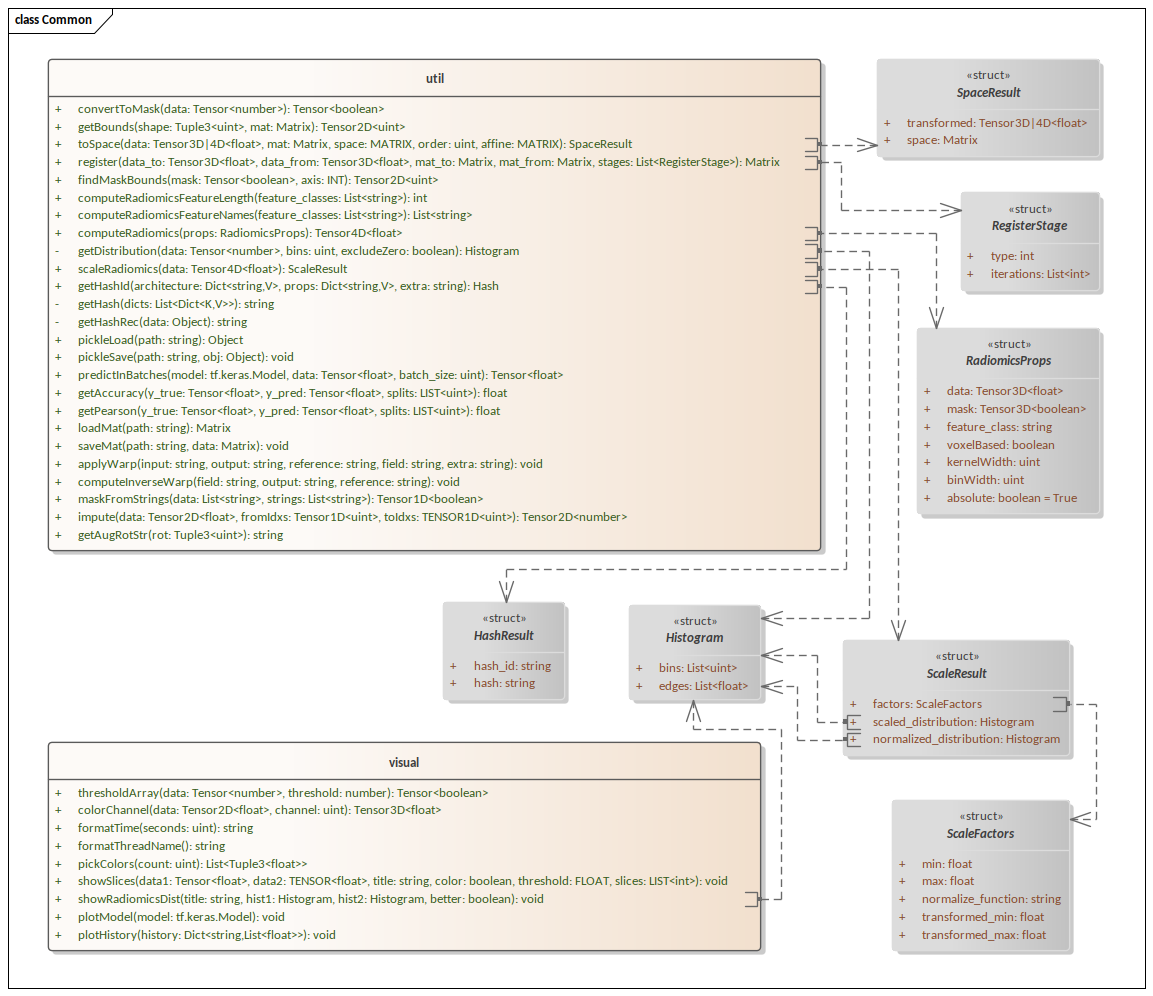
\includegraphics[width=0.7\textwidth]{ClassCommon}
\caption{Class Diagram: Common}
\end{figure}

\section{Preprocessed Data}

Preprocessing the data are composed from the next few high level operations done by the RecordHandler:
\begin{enumerate}
  \item Register some records (not needed for most of them)
  \item Compute all normalized records
  \item Compute the inverse \ac{FNIRT} warp field
  \item Convert native records into our numpy format (apply the affine transformations, merge different sources, etc.)
  \item Compute scaling factors across all native records
  \item Preload native records
  \item Convert normalized records into our numpy format
  \item Compute scaling factors across all normalized records
  \item Preload normalized records
  \item Construct normalized coordinate maps
  \item Warp normalized coordinate maps into native space
  \item Scale and preload coordinate maps
  \item Impute clinical data
\end{enumerate}

After preprocessing, the next set of logical groupings and files are left, split into native and noramlized records:

\begin{figure}[H]
\centering
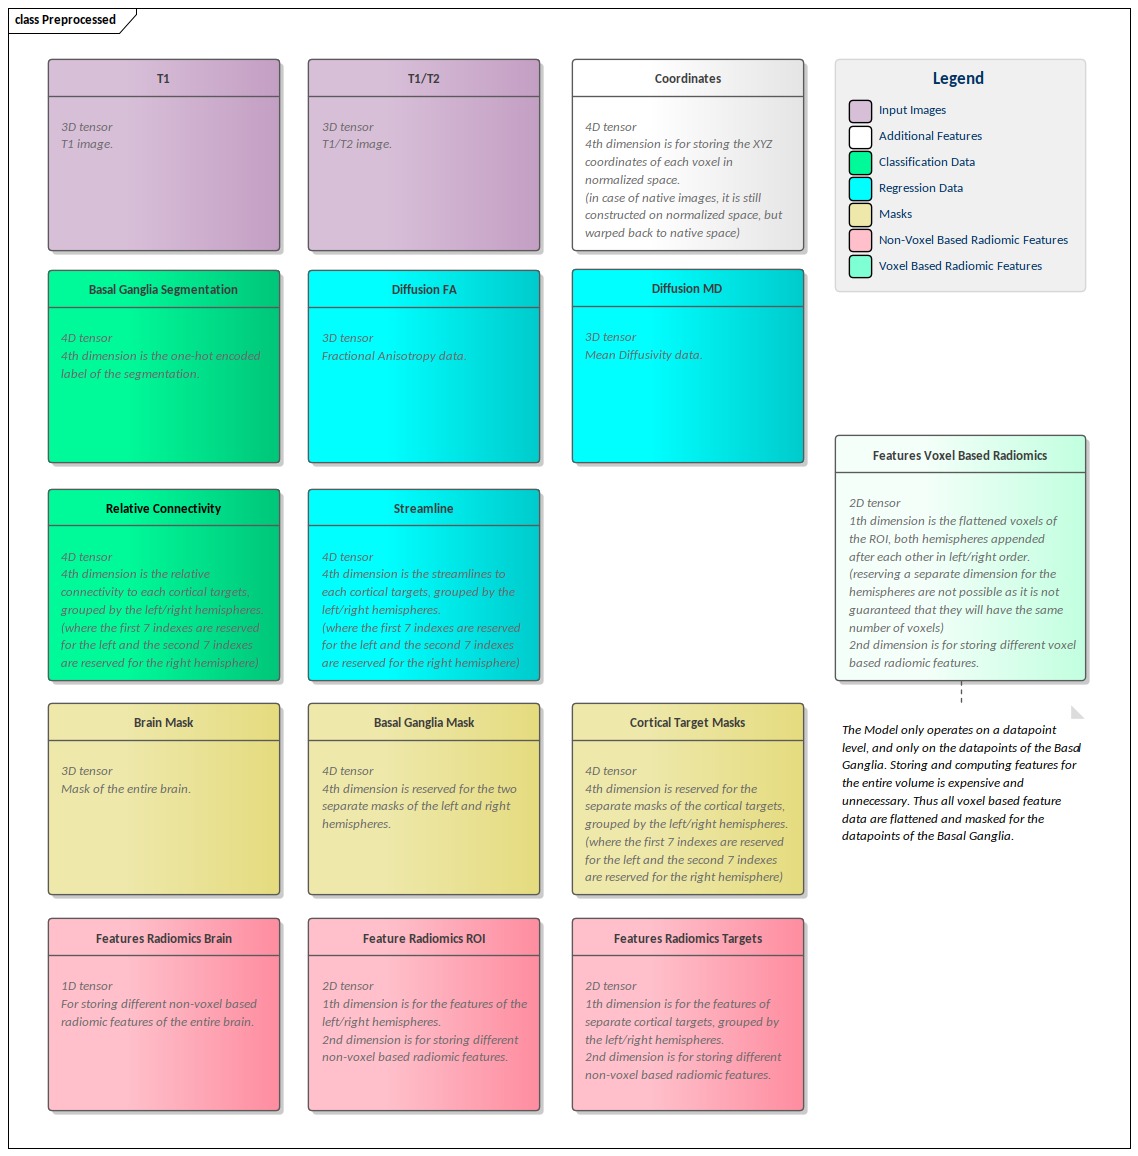
\includegraphics[width=0.7\textwidth]{DataPreprocessed}
\caption{Files: Preprocessed}
\label{fig:files}
\end{figure}

\section{Data Generator}

As this project focuses on only the voxels inside the Basal Ganglia, means the model on a datapoint level is never going to operate outside of that volume.

\begin{figure}[H]
\centering
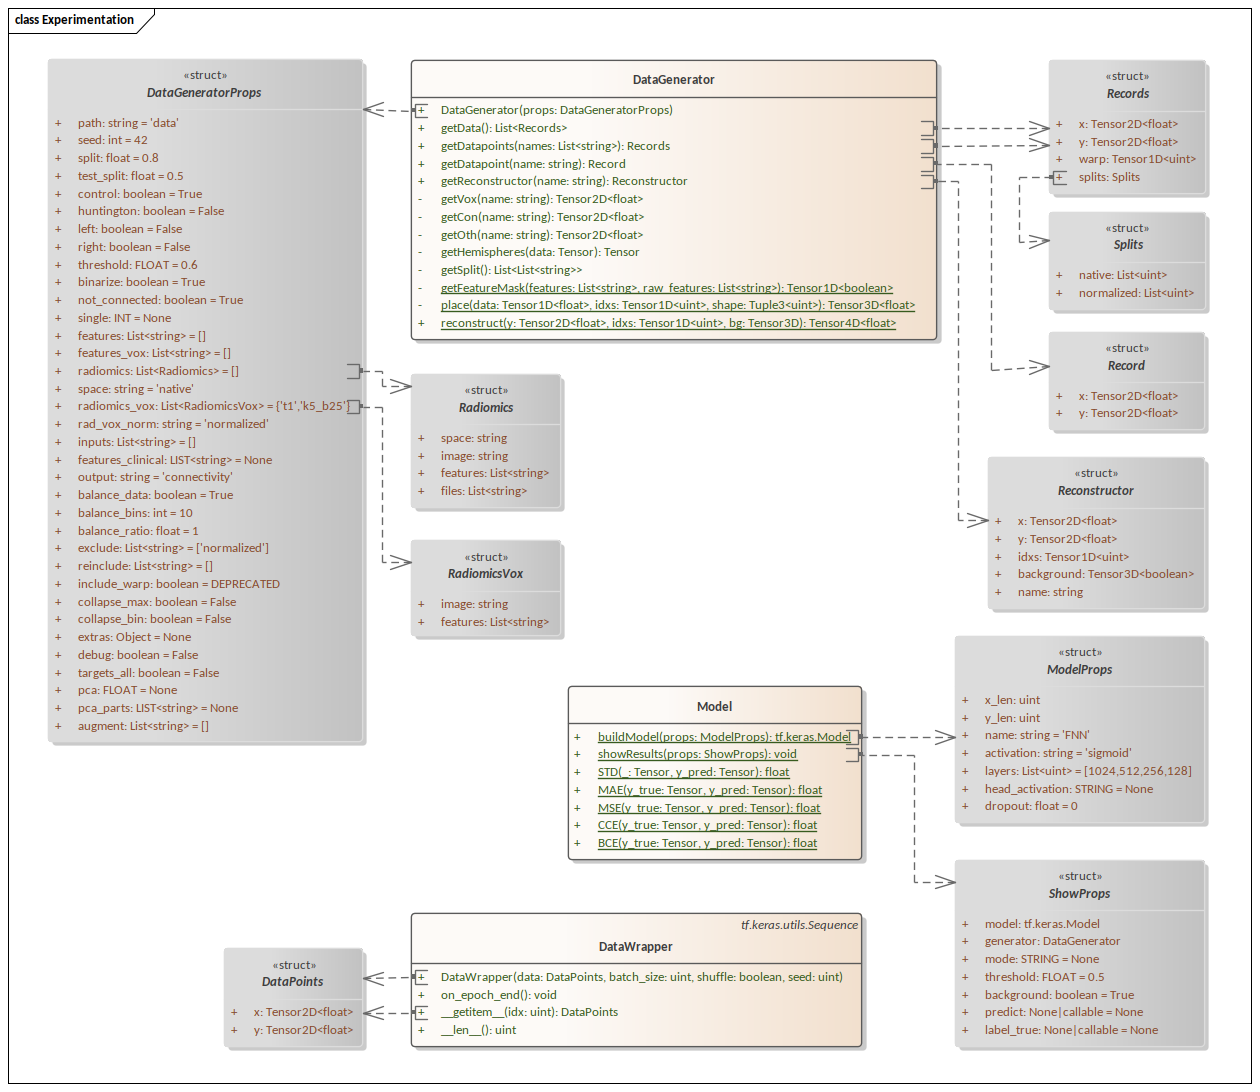
\includegraphics[width=0.7\textwidth]{ClassExperimentation}
\caption{Class Diagram: Experimentation}
\end{figure}

The DataGenerator class is responsible for feeding the Model with data, according to the specifications of the experiments. In order to make this more efficient and fast, loading the entire volume of records from disk can be avoided by 'preloading' the \ac{ROI} from each record. This simply put means that all logical grouping and files specified in \reflink{fig:files}{Figure} are preloaded into 1D and 2D tensors, where the first dimension is the flattened voxels of the \ac{ROI} and the second is whatever layers were stored originally in the last dimension of the spatial data (for example the streamlines of the different traget regions).\par
Computing and persisting the preloaded data vastly speeds up the DataGenerator. Although this has the added consequence that the preloaded data yields a pair of tensors instead of a single volume, as there is differentiation between the left and right hemispere datapoints. And the voxel count in the two hemispheres are not symmetrical, thus the hemisphere differentiation can not be stored as an extra dimension. A design decision was made to store the left and right hemisphere data in separate files.\par
The properties of the DataGenerator provided in its constructor defines the type and format of the generated data.

\begin{longtable}[H]{|L{3cm}|L{3cm}|L{10cm}|}
\hline
\textbf{Value} & \textbf{Type} & \textbf{Description} \\ \hline
path & string & path of the data \\ \hline
seed & int & random seed for the train/val/test splits \\ \hline
split & float & train/all ratio \\ \hline
test\_split & float & test/(test+validation) ratio \\ \hline
control & boolean & include control records \\ \hline
huntington & boolean & include huntington records \\ \hline
left & boolean & include left hemisphere datapoints \\ \hline
right & boolean & include right hemisphere datapoints \\ \hline
threshold & FLOAT & if not None it thresholds the labels by setting the values under the provided threshold to zero; if 0 it re-one-hot encodes the labels (sets the maximum label to 1 and the rest to 0) \\ \hline
binarize & boolean & if thresholded and True, it also sets the labels above the threshold to 1 (and the rest to 0) \\ \hline
not\_connected & boolean & if thresholded and True, it appends an additional 'not connected' label, which complements the sum of the labels per voxel to 1 \\ \hline
single & INT & if not None it only returns the label with the provided index \\ \hline
features & List$<$string$>$ & used non-voxel based radiomics features (emptylist means all) \\ \hline
features\_vox & List$<$string$>$ & used voxel based radiomics features (emptylist means all) \\ \hline
radiomics: List$<$Radiomics$>$ & space: string & space of non-voxel based radiomic features \newline (native/normalized) \\ \cline{2-3}
 & image: string & input image of non-voxel based radiomic features \newline (t1/t1t2) \\ \cline{2-3}
 & features: List$<$string$>$ & list of binning settings of the features \newline (b25, b50, b10r... etc.) \\ \cline{2-3}
 & files: List$<$string$>$ & list of region mask settings of the features \newline (targets/roi/brain) \\ \hline
space & string & space of voxel based radiomic features \newline (native/normalized) \\ \hline
radiomics\_vox: List$<$ & image: string & input image of voxel based radiomic features \newline (t1/t1t2) \\ \cline{2-3}
{   }RadiomicsVox \newline$>$ & features: List$<$string$>$ & list of binning and kernel settings of the features \newline (k5\_b25, k9\_b50, k7\_b10r... etc.) \\ \hline
rad\_vox\_norm & string & use normalization, or only min-max scaling on the voxel based radiomic features (norm/scale) \\ \hline
inps & List$<$string$>$ & additional voxel inputs (t1/t1t2/diffusion/diffusion\_fa/ diffusion\_md/diffusion\_rd) \\ \hline
features\_clin & List$<$string$>$ & additional clinical data inputs (empty array means all) \\ \hline
outp & string & output (connectivity/streamline/basal\_seg/ diffusion\_fa/diffusion\_md/diffusion\_rd) \\ \hline
balance\_data & boolean & enables data balancing \\ \hline
balance\_bins & int & number of bins used for continuous data when balancing \\ \hline
balance\_ratio & float & ratio of the resampling of the difference between each bin and the max bin when balancing (where 0 is unbalanced and 1 is perfectly balanced) \\ \hline
exclude & List$<$string$>$ & can manually add missing groups of records to exclude (t1t2/normalized/basal\_seg/diffusion\_fa) \\ \hline
reinclude & List$<$string$>$ & can manually re-include (append) missing groups of records to the train split (t1t2/normalized/basal\_seg/diffusion\_fa) \\ \hline
debug & boolean & only returns 1/1/1 records for train/val/test when True \\ \hline
augment & List$<$string$>$ & list of record suffixes, used to include augmented records in the training split; for example the suffix '\_5\_0\_0' is used for the rotation augmentation of 5, 0 and 0 degrees on the X, Y and Z axis (naturally these records needs to be computed before using here) \\ \hline
\caption{Data Generator Properties}
\end{longtable}







